% =========================
% CHAPTER 3 — RELATED WORK / STATE-OF-THE-ART (REFINED AFTER REVIEW)
% File: chapter3.tex
%
% NOTE: I kept your structure and changed only what was necessary.
%       I also added more citations. If any citation keys differ from
%       your .bib, just rename the keys accordingly.
% =========================

\chapter{Related Work and the State of the Art} \label{chap:ch3}

This chapter reviews the literature most relevant to \emph{dynamic sampling with multi-agent AUVs using machine learning}.
In line with the course requirements, it is written as a \emph{critical} review: beyond summarising methods, it highlights
assumptions, strengths/limitations, and the implications of each design choice for an onboard-capable and field-deployable
pipeline.

The discussion is organised around the main decisions of a closed-loop adaptive sampling system:
(i) \emph{perceive} and infer what is happening (regimes, events, uncertainty),
(ii) \emph{decide} where/what to sample to maximise utility,
(iii) \emph{coordinate} a team under realistic constraints, and
(iv) \emph{update} a model to close the loop and support replanning.
This structure follows widely used taxonomies in marine robotics and operational oceanography
\parencite{hwang2019auvreview,bernacchi2025closingloop,lermusiaux2007adaptive} and aligns with the broader
\emph{model-driven exploration} perspective, in which numerical forecasts and uncertainty estimates guide robotic sampling
and are, in turn, improved by the collected observations \parencite{mendes2025oceanmodeldriven,curtin2009aosn,duarte2025geostatistical}.

\vspace{1mm}
\noindent\textbf{Evaluation lens used throughout.}
For each work, the review emphasises:
(a) what notion of uncertainty/belief is produced (if any),
(b) what is feasible online/onboard,
(c) what is assumed about communication and coordination,
(d) how heterogeneity and regime boundaries are handled, and
(e) whether the approach closes the loop through explicit model updates and replanning
\parencite{hwang2019auvreview,bernacchi2025closingloop,lermusiaux2007adaptive}.

% ==========================================================
\section{Taxonomy: how the literature closes the loop} \label{sec:taxonomy}

A unifying organising principle for adaptive sampling is the \emph{closed-loop} view:
sensing provides data; diagnosis/inference estimates state, uncertainty, or regimes; adaptation changes actions; and the
collected data updates the model, enabling iterative replanning \parencite{hwang2019auvreview,bernacchi2025closingloop,lermusiaux2007adaptive}.
This perspective is commonly expressed via interacting components such as \emph{sensing}, \emph{diagnosis}, and \emph{adaptation}
(Figure~\ref{fig:pda_loop}). It also appears in operational-oceanography-oriented frameworks where adaptive modelling/data
assimilation and adaptive sampling co-evolve \parencite{lermusiaux2007adaptive,curtin2009aosn}.

\begin{figure}[t]
  \centering
  \begin{tikzpicture}[
      box/.style={draw, rounded corners, align=center, inner sep=6pt, minimum width=27mm},
      arr/.style={-{Latex[length=2.2mm]}, thick},
      lab/.style={font=\scriptsize},
      node distance=10mm and 10mm
    ]
    \node[box] (sense) {Sensing};
    \node[box, right=of sense] (diag) {Diagnosis};
    \node[box, right=of diag] (adapt) {Adaptation};

    \draw[arr] (sense) -- (diag);
    \draw[arr] (diag) -- (adapt);

    \node[draw, dashed, rounded corners, inner sep=6pt, fit=(sense)(diag),
          label={[lab, yshift=2mm]above:\textbf{Perception \& inference}}] (per) {};
    \node[draw, dashed, rounded corners, inner sep=6pt, fit=(adapt),
          label={[lab, yshift=2mm]above:\textbf{Planning \& control}}] (beh) {};
  \end{tikzpicture}
  \caption{A closed-loop view of adaptive sampling: sensing provides observations; diagnosis estimates state/uncertainty/regimes;
  adaptation changes actions accordingly. This loop is widely used to classify adaptive sampling strategies in marine robotics and
  operational oceanography.}
  \label{fig:pda_loop}
\end{figure}

\noindent\textbf{Critical synthesis.}
Two recurring tensions appear across this literature. First, methods with strong probabilistic beliefs
(e.g., full posterior uncertainty over a field) are valuable for decision-making but can be computationally demanding as
domains, horizons, and constraints scale; this motivates approximations, discretisation, or myopic objectives
\parencite{hwang2019auvreview,lermusiaux2007adaptive}. Second, \emph{heterogeneity} is structurally problematic:
coastal regimes and boundaries (fronts/plumes) challenge the assumption that observations can be assimilated into a single
homogeneous model without side-effects, motivating regime-aware inference and update logic
\parencite{fossum2020compact,ge2023watermasses,bernacchi2025closingloop}.

\vspace{1mm}
\noindent Table~\ref{tab:taxonomy_papers} grounds this taxonomy in representative works that are close to the dissertation’s scope.

\begin{table}[H]
  \centering
  \caption{Taxonomy of representative works reviewed in this report. ``Update'' includes data assimilation and analogous posterior refinement (e.g., regression/GPR, belief updates).}
  \label{tab:taxonomy_papers}
  \scriptsize
  \renewcommand{\arraystretch}{1.1}
  \setlength{\tabcolsep}{4pt}
  \begin{tabular}{p{0.20\linewidth} p{0.15\linewidth} p{0.24\linewidth} p{0.17\linewidth} p{0.16\linewidth}}
    \hline
    \textbf{Work} & \textbf{Goal} & \textbf{Model / inference} & \textbf{Planner} & \textbf{Agents \& update} \\
    \hline
    \textcite{hwang2019auvreview} &
    Survey &
    Multiple paradigms &
    Multiple (myopic/MPC/coverage) &
    Single+multi; review (N/A) \\

    \textcite{lermusiaux2007adaptive} &
    Foundation &
    Adaptive modelling + DA + sampling &
    Targeted / adaptive &
    System view; DA concept \\

    \textcite{das2012coordinated} &
    Feature tracking &
    Feature inference / context &
    Coordinated tracking &
    Multi; no explicit DA \\

    \textcite{bernacchi2025closingloop} &
    Forecast improve. &
    Ocean model + uncertainty map &
    PCVRP routing &
    Multi; DA + replanning \\

    \textcite{duarte2025geostatistical} &
    UQ maps &
    Geostatistical UQ + assimilation &
    Uncertainty routing &
    Single; fast assimilation \\

    \textcite{aguiar2018trajectoryopt} &
    Feasibility/cost &
    Flow model (time-varying currents) &
    Traj. optimisation &
    Single/multi; no update \\

    \textcite{fossum2020compact} &
    Regime discovery &
    Dictionary learning + sparse codes &
    Compact-model sampling &
    Typically single; clustering \\

    \textcite{ge2023watermasses} &
    Water-mass class. &
    Probabilistic class model (3D) &
    3D adaptive sampling &
    Single; belief update \\

    \textcite{dalfabbro2025douroplume} &
    Long-term mapping &
    Spatiotemporal GPR + belief &
    Multi-agent RL &
    Multi; GPR update + replanning \\
    \hline
  \end{tabular}
\end{table}


% =========================
% FIGURE — SINGLE vs MULTI (kept, minor caption tightening)
% =========================
\begin{figure}[t]
  \centering
  \begin{tikzpicture}[
      box/.style={
        draw,
        rounded corners,
        align=center,
        font=\scriptsize,
        inner sep=5pt,
        text width=46mm,
        minimum width=46mm,
        minimum height=10mm
      },
      arr/.style={-{Latex[length=2.2mm]}, thick},
      title/.style={font=\scriptsize\bfseries, align=center},
      node distance=8mm and 18mm
    ]

    % --- Left column (single agent / local closed loop) ---
    \node[box] (Tsingle) {$T(t,Z)$\\(field of interest)};
    \node[box, below=of Tsingle] (dyn) {$\dot{x}=f(x,u)$\\$u\in\mathcal{U}$};
    \node[box, below=of dyn] (yhist) {$y(t)$\\(measurements up to $t$)};
    \node[box, below=of yhist] (uSingle) {$u=u(x,t,y(t))$\\(local decision)};

    \draw[arr] (Tsingle) -- (dyn);
    \draw[arr] (dyn) -- (yhist);
    \draw[arr] (yhist) -- (uSingle);

    % --- Right column (multi-agent / coordinated closed loop) ---
    \node[box, right=20mm of Tsingle] (yi) {$y_i(t),\ i=1,\dots,N$\\(distributed measurements)};
    \node[box, below=of yi] (infer) {Diagnosis at $t_k$:\\$\hat{T}_{t_k}$ and $E(t,Z)$\\(regimes/events)};
    \node[box, below=of infer] (alloc) {Allocation / routing:\\$V_i(t_k),\ i=1,\dots,N$\\(tours per vehicle)};
    \node[box, below=of alloc] (uMulti) {$u=u(x,t,V_i(t_k))$\\(tour tracking)};

    \draw[arr] (yi) -- (infer);
    \draw[arr] (infer) -- (alloc);
    \draw[arr] (alloc) -- (uMulti);

    % --- Dashed group boxes ---
    \node[draw, dashed, rounded corners, inner sep=9pt, fit=(Tsingle)(uSingle)] (fitL) {};
    \node[draw, dashed, rounded corners, inner sep=9pt, fit=(yi)(uMulti)] (fitR) {};

    % --- Group titles ---
    \node[title, above=2.5mm of fitL.north] {Single AUV};
    \node[title, above=2.5mm of fitR.north] {Multi-agent};

  \end{tikzpicture}
  \caption{Conceptual distinction between single-agent and multi-agent closed-loop adaptive sampling. In the multi-AUV case,
  decisions are made at coordination times $t_k$ by aggregating distributed measurements, inferring regimes/events, and allocating
  tours to reduce redundancy under communication constraints.}
  \label{fig:single_vs_multi_concept}
\end{figure}

% ==========================================================
\section{Adaptive sampling (single-agent): from ``where to sample'' to ``what to sample''} \label{sec:single_agent}

Many foundational adaptive sampling methods focus on \emph{single-vehicle} decision-making: given a belief about a field or event,
choose the next measurement to maximise a utility function (uncertainty reduction, information gain, or feature-tracking performance)
under motion and mission constraints \parencite{hwang2019auvreview,lermusiaux2007adaptive}. While this dissertation targets multi-agent
settings, single-agent work clarifies the objective functions and the myopic-vs-horizon trade-offs that persist in the team case.

\subsection{Myopic informative planning}
Myopic strategies select the next action by maximising an immediate utility estimate (e.g., local variance reduction).
Their principal advantage is online feasibility: they are responsive to new data and typically lightweight enough for onboard computation
\parencite{hwang2019auvreview}. They are therefore important baselines and often appear as primitives inside receding-horizon schemes.

\textbf{Limitation.} Myopic choices can be systematically suboptimal when dynamics are fast or when travel time matters:
a locally valuable measurement may delay reaching a more influential region, or may ignore time-dependent constraints such as forecast-cycle deadlines.
This issue is emphasised in targeted-observation and adaptive-sampling discussions in operational oceanography \parencite{lermusiaux2007adaptive,curtin2009aosn}.

\subsection{Planning over a horizon (MPC-style) and optimal control}
Horizon-based methods (including MPC-like formulations) improve robustness by accounting for how actions affect \emph{future} information and constraints,
at the cost of increased computation \parencite{hwang2019auvreview}. A complementary view treats adaptive sampling as trajectory optimisation, explicitly
embedding vehicle dynamics and environmental forcing in the cost.

Flow-aware trajectory optimisation is a representative example: time-varying currents are incorporated to reduce time/energy or improve feasibility
\parencite{aguiar2018trajectoryopt}. The appeal is interpretability and explicit constraints; the risk is sensitivity to forecast mismatch, motivating replanning and conservative margins.

\subsection{Model-informed sampling with uncertainty maps (practical onboard route scoring)}
A recurring pragmatic pattern is to build an uncertainty map (from a forecast model, a statistical surrogate, or geostatistics) and treat it as a spatial ``reward'' field
for informative routing. Recent geostatistical uncertainty maps explicitly target real-world onboard feasibility by combining low computational cost with an assimilation step
that changes the uncertainty pattern after incorporating AUV measurements \parencite{duarte2025geostatistical}. This offers a concrete middle ground between
heavy Bayesian field models and purely heuristic strategies.

\subsection{Exploration vs exploitation and feature-driven sampling}
Adaptive sampling inherently trades off exploration (reducing global uncertainty) and exploitation (targeting suspected events/regimes).
The ``what to sample'' question becomes central when the objective is feature-driven (front tracking, plume boundary delineation, or water-mass classification),
where utility is linked to classification confidence or boundary uncertainty rather than to variance alone
\parencite{hwang2019auvreview,ge2023watermasses,das2012coordinated}.

% ==========================================================
\section{Field models, compact representations, and reconstruction} \label{sec:compact_models}

A central design choice in adaptive sampling is the representation of the ocean variable(s) being estimated.
Representations determine: (i) what uncertainty/belief is available for decision-making, (ii) how easily the model can be updated online, and
(iii) how robust updates are in heterogeneous environments.

\subsection{Probabilistic field models and explicit uncertainty}
Probabilistic regression models provide uncertainty estimates that naturally map to sampling utility.
In long-horizon mapping, spatiotemporal Gaussian process regression (GPR) can be maintained and updated as measurements arrive,
allowing the planner to reason about posterior uncertainty and redundancy \parencite{dalfabbro2025douroplume}. The strength is principled
uncertainty; the limitation is scalability without sparsification or local approximations.

\subsection{Geostatistical surrogates for operational uncertainty maps}
Geostatistical approaches can produce spatial predictions and uncertainty with low computational overhead, making them attractive for onboard or near-real-time loops.
In uncertainty-map-driven AUV routing, assimilation of AUV measurements can update both the predicted field and the spatial uncertainty pattern,
explicitly demonstrating the impact of data incorporation on subsequent decisions \parencite{duarte2025geostatistical}. A key limitation is that purely statistical surrogates
may not enforce physical constraints unless coupled to a numerical model or constrained priors.

\subsection{Reduced-order and subspace models}
Reduced-order models compress the field into a low-dimensional subspace, making prediction and update cheaper online.
However, in strongly heterogeneous domains a single global subspace may fit some regimes poorly, motivating regime-conditioned subspaces or mixture-style modelling
\parencite{lermusiaux2007adaptive}.

\subsection{Deep latent models and learned representations}
Learned latent models can represent nonlinear structure and yield compact embeddings.
Their practical adoption hinges on robustness: training data requirements, domain shift (common in coastal settings), and producing calibrated uncertainty.
In parallel, the operational oceanography community has also explored data-driven forecasting at larger scales (seasonal-to-decadal), illustrating the broader trend toward hybrid modelling
\parencite{guo2025orcadl,balaji2022gcmobsolete}. For this dissertation, the key question is not replacing physics-based forecasting, but using ML to extract regime-relevant structure from the data streams that AUVs can realistically collect.

\subsection{Dictionary learning and sparse coding (compact models in practice)}
Dictionary learning with sparse coding is a practical compact modelling approach used for adaptive sampling in marine robotics \parencite{fossum2020compact}.
A high-dimensional observation is represented as a sparse linear combination of learned atoms; the sparse coefficient vector acts as a compact signature.
Fossum \emph{et al.} cluster these sparse codes to discover recurring patterns/regimes, arguing that the codes preserve structure better than coarse summary statistics
and support effective clustering in practice \parencite{fossum2020compact}.

Figure~\ref{fig:fossum_pipeline} summarises how the compact model is embedded in a closed-loop \textit{sense--plan--act} framework, from offline dictionary learning
to online belief update, environment estimation, and replanning.

\begin{figure}[H]
  \centering
  \includegraphics[width=0.95\linewidth]{figures/pipeline_fossun.png}
  \caption{Integration of a compact model into a robotic adaptive sensing loop following a \textit{sense--plan--act} paradigm.
  Reproduced from \textcite{fossum2020compact}.}
  \label{fig:fossum_pipeline}
\end{figure}

\textbf{Critical perspective.}
Sparse codes are attractive for onboard inference because they are compact and can support incremental clustering.
However, the representation is tied to dictionary choice and patching strategy.
Moreover, many compact-model demonstrations use synoptic surface products (e.g., SST patches), whereas this dissertation targets T/S/depth structure:
transferring dictionary learning to CTD profiles requires careful input design (profile windows, derivative features, or learned encoders) and validation that the resulting codes correspond to physically meaningful regimes.

% ==========================================================
\section{Regime detection and water-mass classification} \label{sec:regime_detection}

Regime detection is central to this dissertation because realistic coastal sampling involves transitions between dynamically distinct structures (water masses, fronts, and plume-influenced waters).
A regime-aware pipeline requires: (i) inferring regime identity (ideally as a probabilistic belief) from measurements, and (ii) using this belief to guide planning and to condition model updates.

\subsection{Probabilistic classification from profiles (3D water-mass classification)}
A representative example is 3D adaptive sampling for water-mass classification in frontal systems \parencite{ge2023watermasses}.
In this work, onboard measurements update a probabilistic model over classes across a three-dimensional domain, enabling decisions that target classification performance.
The operational benefit is that the output is a belief distribution rather than a hard label, highlighting ambiguous regions and guiding the vehicle toward informative areas \parencite{ge2023watermasses}.

\textbf{Strengths.} (i) Physically grounded regimes tied to T/S/depth structure; (ii) probabilistic outputs compatible with robust decision-making; (iii) natural handling of regime boundaries via uncertainty in class membership.

\textbf{Limitations.} (i) Sensitivity to feature/model assumptions; (ii) degradation under distribution shift; (iii) the single-vehicle formulation does not directly solve multi-AUV redundancy and coordination.

\subsection{Unsupervised regime discovery with compact representations}
Unsupervised regime discovery is useful when labelled regimes are unavailable or when regimes evolve over time.
Compact-model approaches based on dictionary learning provide a concrete mechanism: encode observations into sparse codes and cluster those codes to discover recurring patterns and regimes \parencite{fossum2020compact}.
Cluster identities can then serve as regime indicators for downstream planning or for gating model updates.

% --- Fossum et al. (IJRR) - PCA / class structure of compact codes ---
\begin{figure}[H]
  \centering
  \includegraphics[width=0.6\linewidth]{figures/clustering.png}
  \caption[Compact-code space visualisation (PCA) in Fossum et al.]{
  Visualisation of an initial classification in compact-code space projected to 2D using PCA, illustrating a cold-to-warm progression.}
  \label{fig:fossum_pca}
\end{figure}

\subsection{Regime cues from ocean currents (flow-derived boundaries)}
As introduced in Chapter~\ref{chap:ch2}, regimes and boundaries are not only expressed by instantaneous T/S gradients,
but can also be suggested by the flow field, which organises transport and mixing into coherent structures
\parencite{weiss2007transportmixing,mcgillicuddy2016mechanisms,mahadevan2016submesoscale}.
The literature typically uses two complementary families of flow diagnostics to delineate dynamically distinct zones.

\textbf{Eulerian indicators} operate on flow snapshots and aim to separate rotation-dominated regions (eddy-like cores)
from strain-dominated regions (filaments/front-like structures). These indicators are attractive for online use due to
their low computational cost, but their reliability depends on the spatial/temporal resolution and noise level of the
available current estimates.

\textbf{Lagrangian diagnostics} characterise transport over a finite time window by integrating particle trajectories,
revealing transport pathways and barriers that naturally partition the domain into regions with distinct mixing behaviour.
This is especially relevant in adaptive sampling because boundaries defined by transport may not coincide with boundaries
defined purely by local T/S gradients.

\textbf{Implications for this dissertation.}
Flow-derived cues are promising to prioritise sampling near moving interfaces even before dense profiling is available,
but they are only as good as the underlying current information and may disagree with water-mass definitions.
Therefore, a practical regime-aware pipeline is likely to benefit from \emph{hybrid} boundary hypotheses that combine
CTD-driven regime belief with flow-derived boundary likelihood, and then test whether this reduces harmful cross-regime
coupling in updates.

 



\subsection{Sequential structure and regime transitions along trajectories}
AUV missions often follow transects where regimes change sequentially. Operationally, recognising when a vehicle crosses a boundary (front/plume edge) is critical both for robust planning and for cautious updates.
Feature-tracking and boundary-focused sampling has a long history in marine robotics, including coordinated sampling of dynamic features \parencite{das2012coordinated} and broader reviews of front/event tracking \parencite{hwang2019auvreview}.
In this dissertation, regime transitions are treated as first-class events to be detected and acted upon.

\subsection{From regime inference to regime-aware planning and updating}
Regime beliefs can be used to: (i) focus sampling near ambiguous boundaries, (ii) allocate team effort across regimes to avoid blind spots, and (iii) condition model updates so local observations do not unduly influence unrelated regimes.
This motivation is consistent with compact models for pattern discovery \parencite{fossum2020compact} and classification-driven adaptive sampling \parencite{ge2023watermasses}.

\begin{figure}[t]
  \centering
  \resizebox{0.78\linewidth}{!}{%
  \begin{tikzpicture}[
      >=Latex,
      axis/.style={->, thick},
      lab/.style={font=\footnotesize},
      pt/.style={circle, fill=black, inner sep=1.4pt}
    ]
    % Axes
    \draw[axis] (0,0) -- (6.4,0) node[lab, below=4pt] {Salinity $S$};
    \draw[axis] (0,0) -- (0,4.4) node[lab, left=4pt] {Temperature $T$};

    % Clusters
    \foreach \x/\y in {1.2/3.2,1.4/3.0,1.1/3.4,1.6/3.1,1.3/3.3} \node[pt] at (\x,\y) {};
    \foreach \x/\y in {3.0/2.2,3.2/2.0,2.9/2.4,3.4/2.1,3.1/2.3} \node[pt] at (\x,\y) {};
    \foreach \x/\y in {4.8/1.2,5.0/1.0,4.7/1.4,5.2/1.1,4.9/1.3} \node[pt] at (\x,\y) {};

    % Regime labels
    \node[lab, anchor=south west] at (1.30,3.45) {Regime A};
    \node[lab, anchor=south]      at (3.20,2.45) {Regime B};
    \node[lab, anchor=north west] at (5.25,1.55) {Regime C};

  \end{tikzpicture}%
  }
  \caption{Conceptual regime separation in T--S space. Clusters represent distinct water-mass or plume-influenced regimes.
  A probabilistic belief over regimes is especially valuable near boundaries, where classification uncertainty is highest.}
  \label{fig:ts_regimes}
\end{figure}

% ==========================================================
\section{Multi-agent adaptive sampling and coordination} \label{sec:multi_agent}

Moving from single-vehicle to multi-vehicle missions increases spatial coverage and supports persistent monitoring, but introduces coordination challenges under intermittent underwater communications
\parencite{hwang2019auvreview,bernacchi2025closingloop,curtin2009aosn}. Multi-agent strategies must manage redundancy, fault tolerance, and decentralised decision-making while delivering measurable gains in scientific utility.

\subsection{Centralised planning and VRP-like formulations}
Centralised planning can allocate targets and generate routes that approximately maximise a global objective under explicit constraints.
A prominent example is the multi-vehicle planner designed to close the loop between prediction and assimilation, formulated as a Prize-Collecting Vehicle Routing Problem (PCVRP) \parencite{bernacchi2025closingloop}.
By associating prizes to candidate sampling sites (e.g., derived from uncertainty maps) and penalising infeasible routes, PCVRP bridges information-driven objectives and operational constraints.

\textbf{Critical perspective.} Centralisation yields coherent global behaviour and explicit redundancy control, but relies on coordination opportunities.
Under sparse connectivity, plans must be computed opportunistically and/or combined with local replanning to handle execution-time deviations (currents, delays, failures).

\begin{figure}[H]
  \centering

  % --- Row 1 ---
  \begin{subfigure}[t]{0.40\textwidth}
    \centering
    \includegraphics[width=\linewidth]{figures/Figure_1.png}
    \caption{Temperature error field (HOPS area) with land mask.}
    \label{fig:bernacchi_err_hops}
  \end{subfigure}
  \hspace*{0.04\textwidth}
  \begin{subfigure}[t]{0.40\textwidth}
    \centering
    \includegraphics[width=\linewidth]{figures/Figure_2.png}
    \caption{Operational area error field after applying mission masks.}
    \label{fig:bernacchi_err_oper}
  \end{subfigure}

  \vspace{2mm}

  % --- Row 2 ---
  \begin{subfigure}[t]{0.40\textwidth}
    \centering
    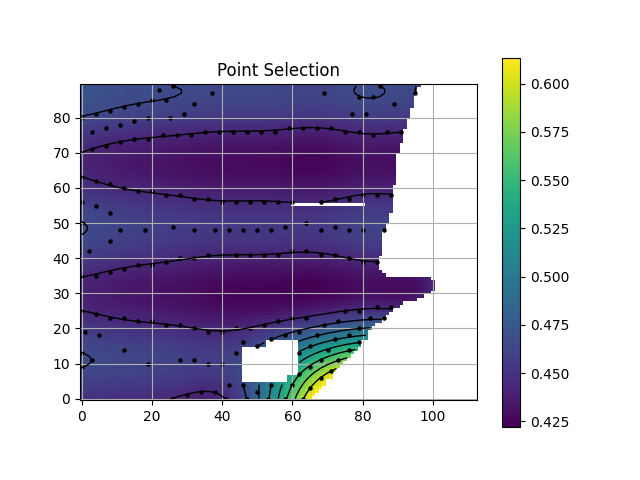
\includegraphics[width=\linewidth]{figures/Figure_3.png}
    \caption{Candidate sampling points overlaid on the error field.}
    \label{fig:bernacchi_points}
  \end{subfigure}
  \hspace*{0.04\textwidth}
  \begin{subfigure}[t]{0.40\textwidth}
    \centering
    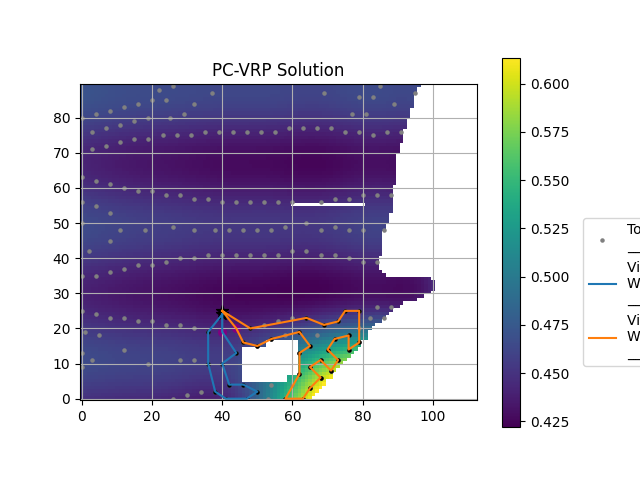
\includegraphics[width=\linewidth]{figures/Figure_4.png}
    \caption{PC-VRP solution (multi-AUV tours) over the same field.}
    \label{fig:bernacchi_pcvrp}
  \end{subfigure}

  \caption{Illustration of a diagnosis-to-routing pipeline in a forecast-improvement setting:
  an error/uncertainty field is masked to define the operational domain, discretised into candidate sites, and then used by a prize-collecting vehicle routing formulation to produce coordinated multi-AUV tours.
  (Recreated/adapted following \textcite{bernacchi2025closingloop}.)}
  \label{fig:bernacchi_pcvrp_pipeline}
\end{figure}

\subsection{Distributed coordination and intermittent communication}
Distributed approaches reduce dependence on continuous connectivity. In practice, hybrid architectures are common: intermittent coordination updates assignments, while vehicles execute local policies between coordination windows \parencite{dalfabbro2025douroplume}.
This improves robustness and reduces communication overhead.

\textbf{Critical perspective.} Avoiding duplication becomes harder without full synchronisation. Distributed methods therefore need mechanisms to discourage overlap (partitioning, task allocation, overlap penalties) and to recover gracefully from missed messages.

\subsection{Autonomy at the team level: organisational and supervisory perspectives}
Beyond route computation, multi-AUV operation often requires higher-level orchestration (roles, delegation, recovery actions, and policies under degraded communications).
Recent work on autonomous robotic organisations for marine operations formalises these aspects, highlighting how organisational structure can improve robustness and scalability in real deployments \parencite{skaugset2025autonomousorg}.
For this dissertation, such perspectives motivate treating coordination as an \emph{architecture} choice (centralised/hybrid/distributed) rather than a single algorithmic component.

\subsection{Learning-based multi-agent control}
Learning-based policies can be attractive when the environment is complex and the decision problem is hard to model exactly.
For long-term plume mapping, multi-agent reinforcement learning combined with spatiotemporal GPR has been proposed, with intermittent coordination via a central entity and online regression updates \parencite{dalfabbro2025douroplume}.

\textbf{Critical perspective.} RL provides flexibility but raises validation concerns: policies must generalise beyond training conditions and remain robust under distribution shift.
Constraint satisfaction and interpretability are typically clearer in optimisation-based approaches (VRP/trajectory optimisation), motivating benchmarking RL against strong optimisation baselines.

% ==========================================================
\section{Planning under time-varying ocean flows} \label{sec:flows}

Currents affect travel time, feasibility, and energy expenditure; therefore flow awareness is a practical requirement in realistic AUV deployments.
Flow-aware trajectory optimisation explicitly accounts for time-varying currents in trajectory generation \parencite{aguiar2018trajectoryopt}, enabling routes that exploit favourable flows or avoid adverse ones.

\textbf{Critical perspective.} Flow-aware optimisation is attractive because constraints are explicit and plans are interpretable, but it can be sensitive to forecast errors.
In multi-agent settings, this sensitivity interacts with coordination: flow-induced delays can break rendezvous windows and increase redundancy if vehicles arrive late to assigned targets.
This motivates iterative replanning and conservative coordination policies in practice \parencite{hwang2019auvreview}.

% ==========================================================
\section{Closing the data loop: model update, assimilation, and forecast improvement} \label{sec:closing_loop}

A key distinction in the literature is between (i) mapping/reconstruction objectives and (ii) \emph{forecast improvement} objectives.
Forecast improvement explicitly targets operational oceanography: observations are valuable insofar as they improve the next nowcast/forecast cycle.
In \emph{closing the data loop} pipelines, a model provides a forecast and uncertainty; a planner selects informative sampling targets; AUVs collect \emph{in situ} data; and assimilation (or an analogous update) yields an improved posterior that supports iterative replanning
\parencite{bernacchi2025closingloop,lermusiaux2007adaptive}.

Recent work demonstrates two practically relevant approaches to operationalising this idea.
First, model-driven exploration pipelines link forecast products, uncertainty maps, and multi-AUV routing in a coherent loop \parencite{mendes2025oceanmodeldriven,bernacchi2025closingloop}.
Second, lightweight geostatistical uncertainty maps show how assimilation can update the spatial uncertainty pattern at low computational cost, supporting shorter cycles and onboard feasibility \parencite{duarte2025geostatistical}.

\textbf{Critical perspective (heterogeneity).}
Forecast improvement is realistic but challenging: it requires integration with a modelling and update pipeline and evaluation metrics that reflect predictive skill.
Moreover, heterogeneous regimes complicate update logic: if a single model is updated indiscriminately using observations collected across dynamically distinct regimes, local improvements can coexist with degraded predictions elsewhere.
This motivates \emph{regime-aware} inference and update strategies, where regime beliefs are used to gate, weight, or separate updates across regimes
\parencite{fossum2020compact,ge2023watermasses,bernacchi2025closingloop}.

% ==========================================================
\section{Where this work fits: gaps and intended contribution} \label{sec:gap_contribution}

The reviewed literature provides strong building blocks for closed-loop adaptive sampling, but exposes gaps directly aligned with the dissertation’s problem statement (sampling across \emph{dynamically distinct regimes} and using ML to learn regime structure from data):

\begin{itemize}
  \item \textbf{Regime inference is not routinely integrated with multi-AUV planning.}
  Probabilistic regime classification from profiles is well motivated \parencite{ge2023watermasses}, and compact representations support unsupervised regime discovery \parencite{fossum2020compact}, but these elements are rarely combined with multi-agent routing in a single end-to-end pipeline.

  \item \textbf{Closing the loop is often demonstrated either with strong modelling assumptions or with limited regime awareness.}
  Forecast-improvement pipelines link uncertainty maps, routing, and assimilation \parencite{bernacchi2025closingloop,mendes2025oceanmodeldriven}, and geostatistical approaches offer operationally light updates \parencite{duarte2025geostatistical}.
  However, explicit mechanisms to prevent harmful cross-regime coupling in updates are still limited in multi-agent settings.

  \item \textbf{Coordination under intermittent communications remains a dominant constraint.}
  VRP-style formulations offer practical constraint handling and explicit redundancy control \parencite{bernacchi2025closingloop}, while intermittent coordinator architectures and learning-based schemes improve robustness \parencite{dalfabbro2025douroplume}.
  Systematic comparisons under common metrics (information gain, forecast improvement, redundancy, operational cost) remain relatively scarce \parencite{hwang2019auvreview}.
\end{itemize}

Based on these observations, the dissertation will pursue a regime-aware, closed-loop pipeline for multi-AUV adaptive sampling built from four elements:

\begin{itemize}
  \item \textbf{Regime inference from T/S/depth measurements} using compact representations and probabilistic beliefs inspired by water-mass classification and compact-model approaches \parencite{ge2023watermasses,fossum2020compact}.

  \item \textbf{Informative objectives that remain operational} by connecting uncertainty/forecast-error proxies to routing decisions (including uncertainty maps and model-driven exploration patterns) \parencite{bernacchi2025closingloop,duarte2025geostatistical,mendes2025oceanmodeldriven}.

  \item \textbf{Multi-agent coordination robust to sparse communications} by combining VRP-like global allocations (when possible) with local execution policies between coordination windows \parencite{bernacchi2025closingloop,dalfabbro2025douroplume,skaugset2025autonomousorg}.

  \item \textbf{Flow-aware feasibility and cost modelling} to keep routes realistic under time-varying currents \parencite{aguiar2018trajectoryopt}.
\end{itemize}

% ==========================================================
\section{Summary} \label{sec:ch3_summary}

This chapter reviewed state-of-the-art approaches for closed-loop adaptive sampling and highlighted the trade-offs that matter for an onboard-capable multi-AUV system.
Survey taxonomies clarify how sensing, diagnosis, and adaptation interact \parencite{hwang2019auvreview}.
Operational oceanography perspectives motivate closing the loop between modelling, assimilation, and sampling \parencite{lermusiaux2007adaptive,curtin2009aosn}.
Compact representations such as sparse codes support regime-like structure discovery and lightweight inference \parencite{fossum2020compact}, while probabilistic water-mass classification illustrates how profile-driven regime beliefs can be updated online \parencite{ge2023watermasses}.
Forecast-improvement pipelines can be operationalised via VRP-like multi-AUV planning linked to uncertainty maps and assimilation \parencite{bernacchi2025closingloop,mendes2025oceanmodeldriven}, and geostatistical uncertainty maps offer a complementary route to fast, operational updates \parencite{duarte2025geostatistical}.
Finally, long-horizon multi-agent plume mapping demonstrates persistent monitoring under intermittent coordination \parencite{dalfabbro2025douroplume}.
Across these works, the main gap motivating this dissertation is the limited integration of \emph{regime awareness} with \emph{multi-agent coordination} and \emph{flow-aware, forecast-improving closed-loop updates} in a single, comparably evaluated pipeline.
